%%%%%%%%%%%%%%%%%%%%%%%%%%%%%%%%%%%%%%%%%
% Jacobs Landscape Poster
% LaTeX Template
% Version 1.1 (14/06/14)
%
% Created by:
% Computational Physics and Biophysics Group, Jacobs University
% https://teamwork.jacobs-university.de:8443/confluence/display/CoPandBiG/LaTeX+Poster
% 
% Further modified by:
% Nathaniel Johnston (nathaniel@njohnston.ca)
%
% This template has been downloaded from:
% http://www.LaTeXTemplates.com
%
% License:
% CC BY-NC-SA 3.0 (http://creativecommons.org/licenses/by-nc-sa/3.0/)
%
%%%%%%%%%%%%%%%%%%%%%%%%%%%%%%%%%%%%%%%%%

%----------------------------------------------------------------------------------------
%	PACKAGES AND OTHER DOCUMENT CONFIGURATIONS
%----------------------------------------------------------------------------------------

\documentclass[final]{beamer}
\usepackage{ragged2e} 
\usepackage[scale=1.24]{beamerposter} % Use the beamerposter package for laying out the poster

\usetheme{confposter} % Use the confposter theme supplied with this template

\setbeamercolor{block title}{fg=MidnightBlue,bg=white} % Colors of the block titles
\setbeamercolor{block body}{fg=black,bg=white} % Colors of the body of blocks
\setbeamercolor{block alerted title}{fg=Maize,bg=dblue!70} % Colors of the highlighted block titles
\setbeamercolor{block alerted body}{fg=black,bg=dblue!10} % Colors of the body of highlighted blocks
% Many more colors are available for use in beamerthemeconfposter.sty

%-----------------------------------------------------------
% Define the column widths and overall poster size
% To set effective sepwid, onecolwid and twocolwid values, first choose how many columns you want and how much separation you want between columns
% In this template, the separation width chosen is 0.024 of the paper width and a 4-column layout
% onecolwid should therefore be (1-(# of columns+1)*sepwid)/# of columns e.g. (1-(4+1)*0.024)/4 = 0.22
% Set twocolwid to be (2*onecolwid)+sepwid = 0.464
% Set threecolwid to be (3*onecolwid)+2*sepwid = 0.708

\newlength{\sepwid}
\newlength{\sepwidd}
\newlength{\onecolwid}
\newlength{\onecolwidd}
\newlength{\twocolwid}
\newlength{\threecolwid}
\setlength{\paperwidth}{48in} % A0 width: 46.8in
\setlength{\paperheight}{36in} % A0 height: 33.1in
\setlength{\sepwid}{0.024\paperwidth} % Separation width (white space) between columns
\setlength{\onecolwid}{0.22\paperwidth} % Width of one column
\setlength{\onecolwidd}{0.24\paperwidth} % Width of one column
\setlength{\twocolwid}{0.464\paperwidth} % Width of two columns
\setlength{\threecolwid}{0.708\paperwidth} % Width of three columns
\setlength{\topmargin}{-0.5in} % Reduce the top margin size
\setlength{\sepwidd}{0.004\paperwidth}
%-----------------------------------------------------------


\addtobeamertemplate{block begin}{}{\justifying}  %new code



\usepackage{graphicx}  % Required for including images

\usepackage{booktabs} % Top and bottom rules for tables

%----------------------------------------------------------------------------------------
%	TITLE SECTION 
%----------------------------------------------------------------------------------------

\title{Parallel pathfinding for Amazon's Prime Air UAVs} % Poster title

\author{Stephan Boettcher} % Author(s)

\institute{Department of Computational Science and Engineering, Georgia Institute of Technology} % Institution(s)

%----------------------------------------------------------------------------------------

\begin{document}

\addtobeamertemplate{block end}{}{\vspace*{2ex}} % White space under blocks
\addtobeamertemplate{block alerted end}{}{\vspace*{2ex}} % White space under highlighted (alert) blocks

\setlength{\belowcaptionskip}{2ex} % White space under figures
\setlength\belowdisplayshortskip{2ex} % White space under equations

\begin{frame}[t] % The whole poster is enclosed in one beamer frame

\begin{columns}[t] % The whole poster consists of three major columns, the second of which is split into two columns twice - the [t] option aligns each column's content to the top

\begin{column}{\sepwid}\end{column} % Empty spacer column

\begin{column}{\onecolwid} % The first column

%----------------------------------------------------------------------------------------
%	OBJECTIVES
%----------------------------------------------------------------------------------------

\begin{alertblock}{Objectives}
The objective of this project was to:
\begin{itemize}
\item Establish baseline performance of the A* pathfinding algorithm
\item Determine how to generate a large number of optimal paths as fast as possible
\end{itemize}

\end{alertblock}

%----------------------------------------------------------------------------------------
%	INTRODUCTION
%----------------------------------------------------------------------------------------

\begin{block}{Introduction}
Amazon Prime Air\cite{amazon} was announced December 2013 as a way to deliver packages within 30 minutes of ordering. This will be achieved through the use of small unmanned aerial vehicles (UAV). The Amazon Prime Air project places restrictions on which customers are able to utilize this service, usually based on a geographic radius from a supply warehouse. These UAVs currently have small payload capacities and limited range due to battery power density restraints. To achieve peak efficiency, these UAVs will need to fly from the warehouse to their delivery location following an optimal path. In a dense urban environment, such as Los Angeles as seen in Figure , airspace restrictions are fluid and subject to change over the course of a day. A pathfinding algorithm must be able to handle these changes while still being able to generate a large number of routes quickly.

\end{block}

%------------------------------------------------

\begin{figure}
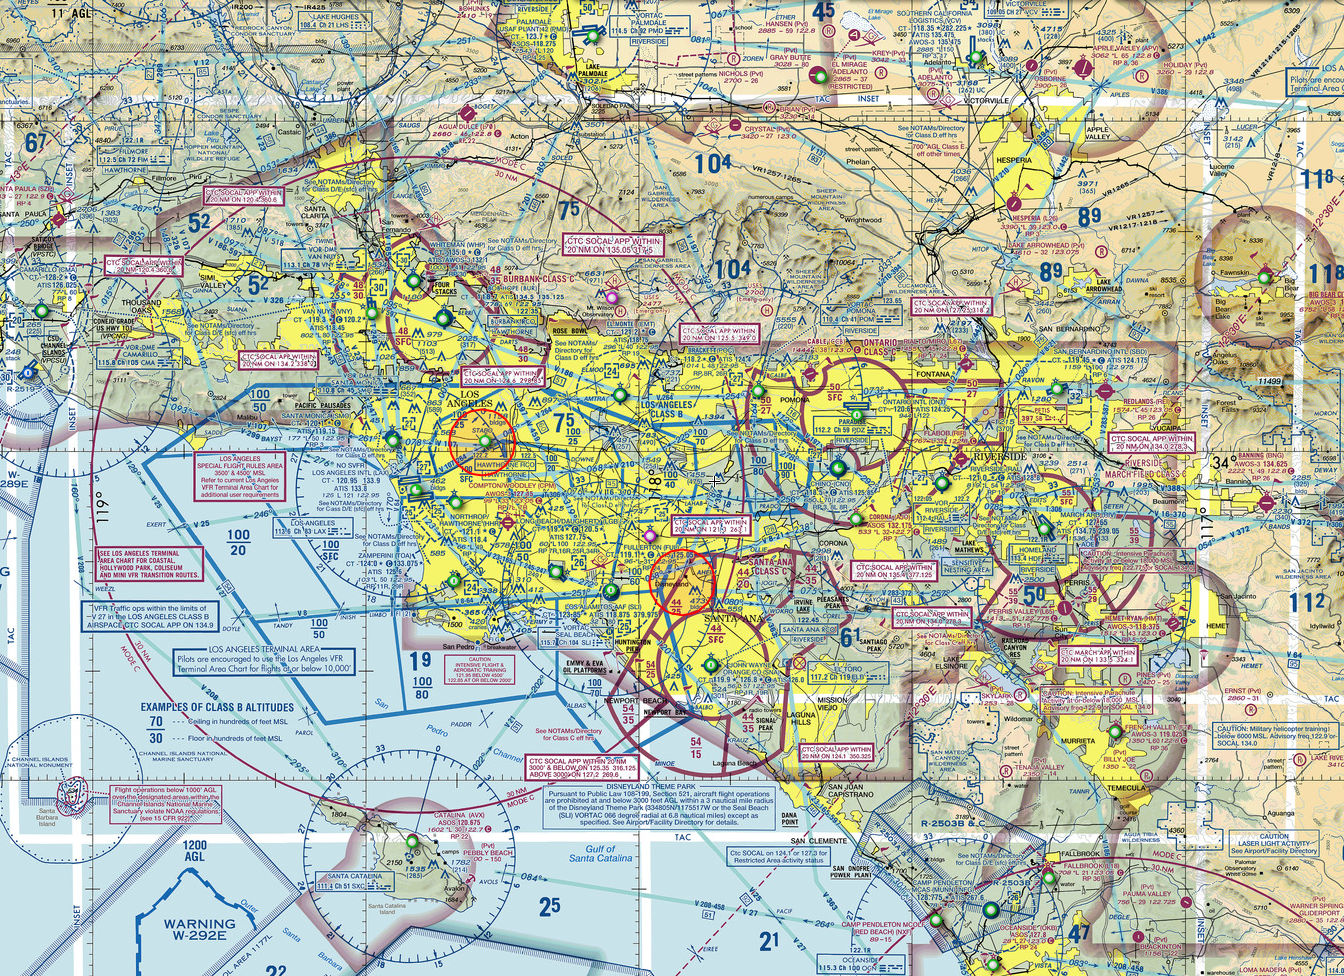
\includegraphics[width=0.99\linewidth]{LAX.png}
\caption{FAA airspace surrounding Los Angeles}
\end{figure}

%----------------------------------------------------------------------------------------

\end{column} % End of the first column

    \begin{column}{\sepwid}\end{column} % Empty spacer column

\begin{column}{\twocolwid} % Begin a column which is two columns wide (column 2)

%   
%    
%    \begin{column}{\onecolwid}\vspace{-.6in} % The first column within column 2 (column 2.1)

%
%----------------------------------------------------------------------------------------
%	METHODS
%----------------------------------------------------------------------------------------

\begin{block}{Methods}
 \begin{columns}[t,totalwidth=\twocolwid] % Split up the two columns wide column
 \begin{column}{\onecolwidd} % The first column within column 2 (column 2.1)
 
 {\parskip0pt\par}
  \ifbeamercolorempty[bg]{block title}
  {}
  {\ifbeamercolorempty[bg]{block body}{}{\nointerlineskip\vskip-0.5pt}}
  \usebeamerfont{block body}
  \vskip-0.5cm
  \begin{beamercolorbox}[colsep*=0ex,vmode]{block body}
  \justifying

 A single path can be generated quickly using an algorithm similar to the Parallel Ripple Search or the Fringe Search\cite{Brand}\cite{Botea}. Unfortunately these two methods utilize all of the system computing resources. Conversely, it is possible to spawn off one path per thread and batch process the paths using a slower serial algorithm. This method results in all threads being dedicated to batch processing. Peak efficiency is achieved with a blend of these two paradigms.
  \newline
The following steps were taken for analysis:
\begin{enumerate}
\item Generate 6 maps for benchmarking suite
\item Batch process A* algorithm
\item Parallelize and batch process A* algorithm
\item Used MPI to perform distributed parallel batch processing on A* algorithm
\item Parallelized Fringe Search method
\item Determined optimality lost by Fringe Search method
\end{enumerate}
  \end{beamercolorbox}

\end{column}
  % \begin{column}{\sepwidd}\end{column} % Empty spacer column
 \begin{column}{\onecolwidd}
  {\parskip0pt\par}
  \ifbeamercolorempty[bg]{block title}
  {}
  {\ifbeamercolorempty[bg]{block body}{}{\nointerlineskip\vskip-0.5pt}}
  \usebeamerfont{block body}
  \vskip-0.5cm
  \begin{beamercolorbox}[colsep*=0ex,vmode]{block body}
  \justifying
 \begin{center}
 
 
 
\begin{figure}

\includegraphics[width=0.85\linewidth]{Run_3.png}
\caption{Sample path output from A* algorithm}
\end{figure}
\end{center}




  \end{beamercolorbox}
\end{column}

\end{columns}
\end{block}

%----------------------------------------------------------------------------------------

%    \end{column} % End of column 2.2
%    
%    \end{columns} % End of the split of column 2 - any content after this will now take up 2 columns width

%----------------------------------------------------------------------------------------
%	IMPORTANT RESULT
%----------------------------------------------------------------------------------------


%----------------------------------------------------------------------------------------
%	RESULTS
%----------------------------------------------------------------------------------------

\begin{block}{Results}
 \begin{columns}[t,totalwidth=\twocolwid] % Split up the two columns wide column
 \begin{column}{\onecolwidd} % The first column within column 2 (column 2.1)


\begin{figure}
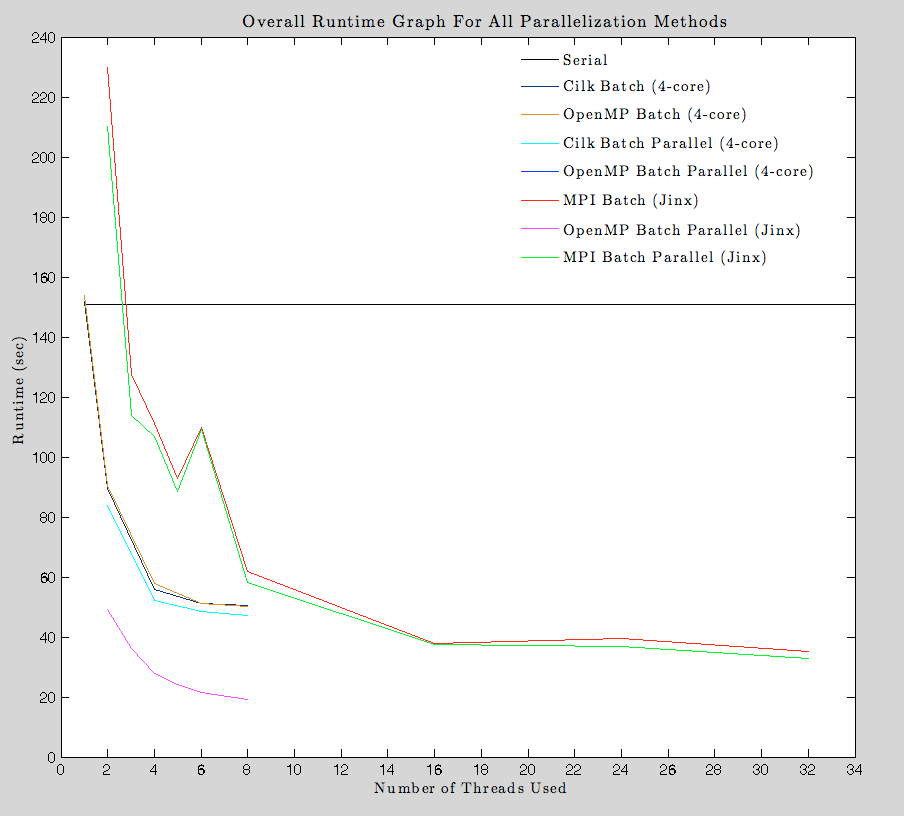
\includegraphics[width=0.9\linewidth]{Alldata.png}
\caption{Final results of parallelization methods}
\end{figure}


\end{column} % End of column 2.2
%\begin{column2}{\sepwidd}\end{column2} % Empty spacer column
 \begin{column}{\onecolwidd}

The overall results were:
\begin{itemize}
\item The OpenMP code running in batch parallel was able to achieve a 8x speedup on a 6 core Jinx cluster 
\item MPI configurations were slower than expected due to the large number of small messages required for scenario setup and result collection
\item Cilk and OpenMP achieved equivalent speedups 
\item OpenMP is able to integrate with other parallelization methods such as MPI, unlike Cilk
\item Paths created by the Fringe Search algorithm were up to 10\% longer than A* algorithms. This corresponds to longer flight times for the UAVs
\end{itemize}

%----------------------------------------------------------------------------------------

    \end{column} % End of column 2.2
    
    \end{columns} % End of the split of column 2
\end{block}


\begin{alertblock}{}
OpenMP A* algorithm in a batch parallel configuration was the fastest method to generate 1000 paths. 
\end{alertblock} 

\end{column} % End of the second column

\begin{column}{\sepwid}\end{column} % Empty spacer column

\begin{column}{\onecolwid} % The third column

%----------------------------------------------------------------------------------------
%	CONCLUSION
%----------------------------------------------------------------------------------------

\begin{block}{Conclusion}

 A linear speedup of the runtimes was achieved under restrained conditions and a large number of complex paths were able to be calculated in a short timeframe. While it is somewhat difficult to drastically parallelize this code while still maintaining optimality, sufficient parallelization options were available to achieve large speedups. The effects of MPI message size, quantity and type were investigated, as were the effects of combining multiple parallelization paradigms. Ultimately, the economic limits and physical constraints surrounding the use of UAVs as a package delivery system dictated the largest constraints on the project. Had the path generation runtimes been longer than the added flight time of a UAV on a suboptimal path, other path-finding algorithms could have been utilized and parallelized. Thus, a parallelized A* algorithm will be the ideal method for Amazon Prime Air to generate the most efficient UAV routes.

\end{block}

%----------------------------------------------------------------------------------------
%	ADDITIONAL INFORMATION
%----------------------------------------------------------------------------------------

%\begin{block}{Future Research}
%
%Optimizing Further gains may come from optimizing the message types and sizes in the MPI portion of the code. 
%
%\end{block}

%----------------------------------------------------------------------------------------
%	REFERENCES
%----------------------------------------------------------------------------------------

\begin{block}{References}

%\nocite{*} % Insert publications even if they are not cited in the poster
\small{\bibliographystyle{unsrt}
\begin{thebibliography}{99} 
\bibitem{amazon} "Amazon Prime Air". Retrieved December , 2014 
\bibitem{Brand} S. Brand,  and R.  Bidarra, Multi-core scalable and efficient pathfinding with Parallel Ripple Search. Comp. Anim. Virtual Worlds, 23: 73�85. doi: 10.1002/cav.1427, 2012
\bibitem{Botea} A. Botea, "Near optimal hierarchical path-finding", Journal of Game Development , vol 1 , no , p.7 - 28, 2004.
\bibitem{Cohen} D. Cohen and M. Dallas, "Implementation of parallel path finding in a shared memory architecture", Dept. CS, Rensselaer Polytech Inst, Troy, NY, 2010. 
%\bibitem{Inam} R. Inam, "A* algorithm for multi-core graphics processors", M.S. Thesis, Dept. Comput. Eng, Chalmers Tech Inst, G\"oteborg 2009. 

 \end{thebibliography}
}
\end{block}

%----------------------------------------------------------------------------------------
%	ACKNOWLEDGEMENTS
%----------------------------------------------------------------------------------------
%
%\setbeamercolor{block title}{fg=red,bg=white} % Change the block title color
%
%\begin{block}{Acknowledgements}
%
%\small{\rmfamily{Nam mollis tristique neque eu luctus. Suspendisse rutrum congue nisi sed convallis. Aenean id neque dolor. Pellentesque habitant morbi tristique senectus et netus et malesuada fames ac turpis egestas.}} \\
%
%\end{block}

%----------------------------------------------------------------------------------------
%	CONTACT INFORMATION
%----------------------------------------------------------------------------------------

\setbeamercolor{block alerted title}{fg=black,bg=norange} % Change the alert block title colors
\setbeamercolor{block alerted body}{fg=black,bg=white} % Change the alert block body colors

\begin{alertblock}{Contact Information}

\begin{itemize}
%\item Web: \href{http://www.university.edu/smithlab}{http://www.university.edu/smithlab}
\item Email: \href{mailto:sboettcher3@gatech.edu}{sboettcher3@gatech.edu}
\end{itemize}

\end{alertblock}

\begin{center}


\includegraphics[width=\linewidth]{cc_logo.png}

\end{center}

%----------------------------------------------------------------------------------------

\end{column} % End of the third column

\end{columns} % End of all the columns in the poster

\end{frame} % End of the enclosing frame

\end{document}
